\subsubsection{CYBEX}

Cybersecurity Information Exchange Framework (CYBEX) provee un formato y un 
framework para asegurar el intercambio de información de seguridad y permitir la 
automatización del intercambio. CYBEX se centra en el intercambio de información 
de seguridad entre organizaciones como se ve en la figura 2. Como se ve,
CYBEX no busca dar una forma para obtener o utilizar información de seguridad.

\begin{figure}[ht!]
  \centering
    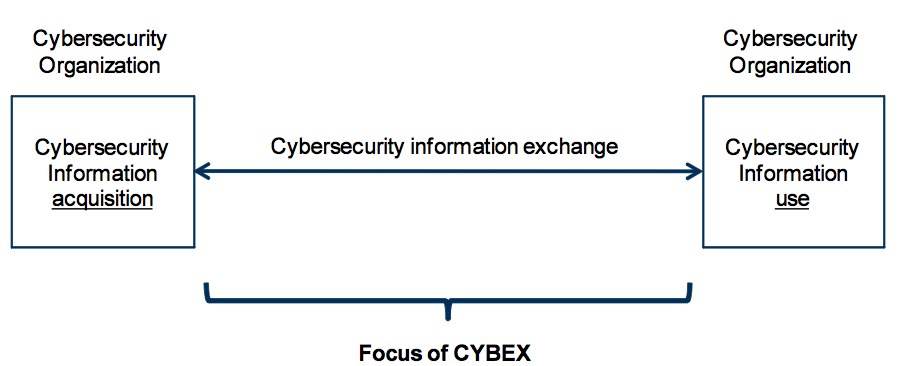
\includegraphics[width=150mm]{./images/cybex.png}
    \caption{CYBEX \protect\cite{b1}}
\end{figure}

El framework provee un entorno donde el conocimiento proveniente de reportes, 
testeo y experiencias es utilizado para crear y actualizar la información de 
debilidades y vulnerabilidades. Por lo tanto, puede ser utilizado con el estado 
del sistema para medir y mejorar la seguridad de éste. También puede ser 
utilizado para crear extensiones que permitan detección de malware o la 
automatización de información referente a software, servicios y sistemas. 

En el diseño de CYBEX se consideran cinco bloques funcionales: Information 
Description, Information Discovery, Information Query, Information Assurance e 
Information Transport. El bloque Information Description estructura la 
información de cyber seguridad con el propósito de intercambiarla, el bloque 
information discovery identifica y descubre la información de seguridad y las 
entidades. El bloque information query es utilizado para los pedidos y 
respuestas de información de seguridad. El bloque information assurence asegura 
la validez de la información y el bloque informatiosn transport intercambia la 
información en la red.

Cada bloque funcional consiste de distintas especificaciones como las mostradas 
en la tabla 1. Como se puede ver en la tabla, CYBEX utiliza standards y que como 
CYBEX es creado en cooperación con los creadores de cada uno de esos estándares 
se puede aumentar la utilidad y compatibilidad de CYBEX con dichos estándares. 
De esta forma los usuarios son capaces de usar CYBEX con productos ya 
disponibles.

AGREGAR LA TABLA DE CYBEX

\paragraph{Information Description Block}

Este bloque estructura la información para el intercambio y provee los formatos 
y lenguajes necesarios para describirlo. CYBEX se define por medio de dominios 
de operación, los roles requeridos en cada uno de dichos dominios y la 
información que cada uno de esos roles maneja. Algunos elementos utilizados son 
IODEF, CVE, CWE u OVAL.

\paragraph{Information Discovery Block}

Este bloque identifica información de seguridad y entidades. Se proveen dos 
paradigmas para el descubrimiento de servicios e información, descubrimiento 
centralizado o de-centralizado.

En el descubrimiento centralizado se indexa la información en un árbol 
jerárquico, de esta forma se puede buscar recorriendo dicho árbol. De está forma





